\chapter{Kontrolinterface}
Nedenfor følger design af software til Kontrolinterfacet. Dette er lavet på baggrund af kravspecifikation og systemarkitektur. 
\subsection{Modulets ansvar}
Kontrolinterfacet er brugerens primære kontaktflade til systemet. Programmet indeholder en brugergrænseflade der opfylder kravene i Kravspecifikationen. Her kan der også ses en prototype på den grafiske brugergrænseflade.
Kontrolinterfacet står for at modtage inputs fra brugeren. Disse inputs sendes som kommandoer til Styringsmodulet. Det er også herfra at Kontrolinterfacet modtager de værdier, som sidenhen vises på den grafiske brugergrænseflade. Kontrolinterfacet står også for kommunikationen til den eksterne database. Her sendes en række parametre om skibet og dets status.

\subsection{State machine diagram}
Designet af Kontrolinterfacet tager udgangspunkt i arkitekturen fremstillet i artefaktet Systemarkitektur. Her blev der fremstillet et state machine for Kontrolinterfacet. State machinet var simplificeret og er i designfasen blevet udvidet. Resultatet ses i figur \ref{fig:stm_detaljeret}.\\
Figuren beskriver hvilke stadier programmet kan befinde sig i og sammenhængen imellem dem.\\
Størstedelen af kontrolinterfacets levetid foregår i et ventestadie hvor der afventes enten et brugerinput eller et timeout. Begge scenarier afføder et behov for kommunikation med styringsmodulet. \\
Hvis der har været et timeout skal der hentes værdier fra Styringsmodulet hvorefter Databasen opdateres.\\
Hvis der har været et brugerinput skal Kontrolinterfacet blot have en bekræftigelse fra Styringsmodulet på at kommandoen er modtaget.\\

\begin{figure}[htbp]
\centering
\label{fig:stm_detaljeret}
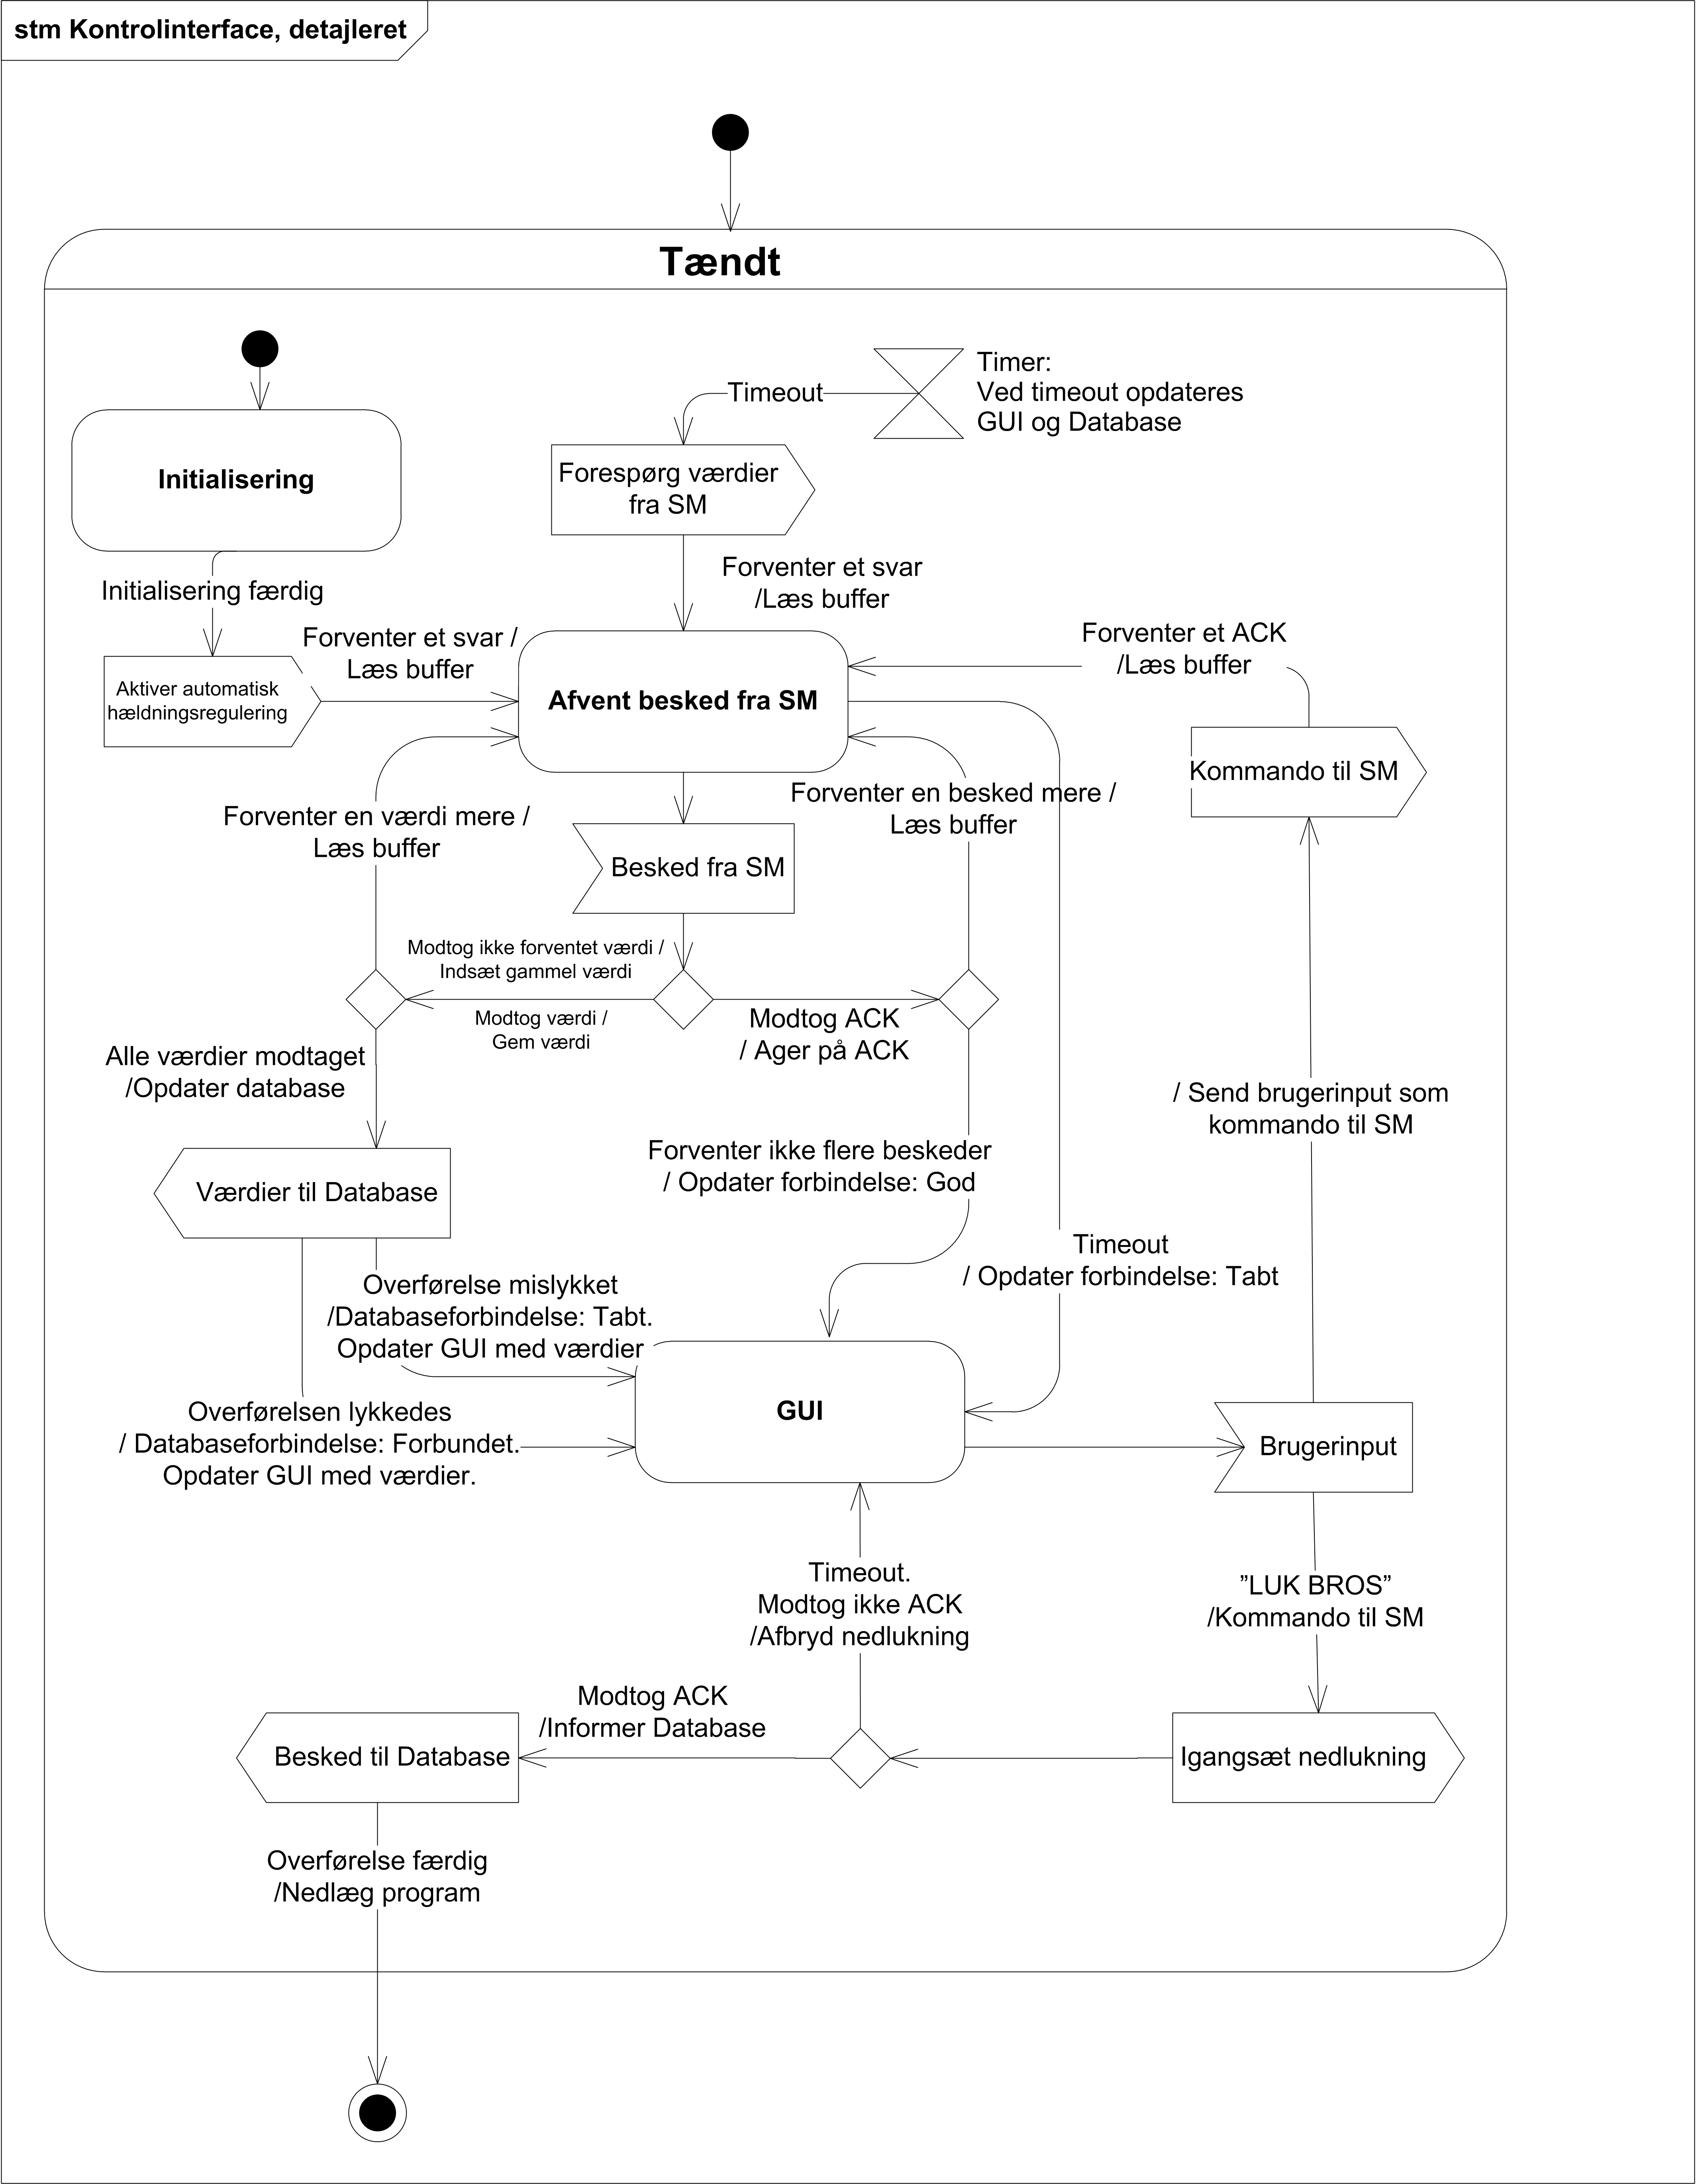
\includegraphics[width=1\textwidth]{billeder/GUI/STM_KI_DETALJERET}
\caption{På figuren ses det detaljerede state machine diagram for Kontrolinterfacet}
\end{figure}

\subsection{Klassediagram}
Således er det videre skridt at udarbejde et klassediagram for programmet. Her anvendes klassediagrammer. Klassediagrammet er ligesom state machines først lavet i en simplificeret version og dernæst i en detaljeret. Den første kan ses på figur \ref{fig:kd_simpel}.

Klassediagrammet på figur \ref{fig:kd_simpel} afspejler et system designet med forbillede i det samlede system. Dette er gjort for at trække på de løsninger der er fundet i forbindelse med det fulde system. Her ses det hvordan hovedklassen er Kontrolinterfacet. Alt andet oprettes enten direkte af Kontrolinterface-klassen eller af en klasse oprettet af samme. Kontrolinterfacet har kun kontakt til brugergrænsefladen (MainWindow), Styringsmodulet og DataServer. Kommunikationen mellem Kontrolinterface-klassen og Styringsmodul spejler den kommunikation der er imellem de fysiske blokke Kontrolinterface og Styringsmodul i det samlede system.\\

\begin{figure}[htbp]
\centering
\label{fig:kd_simpel}
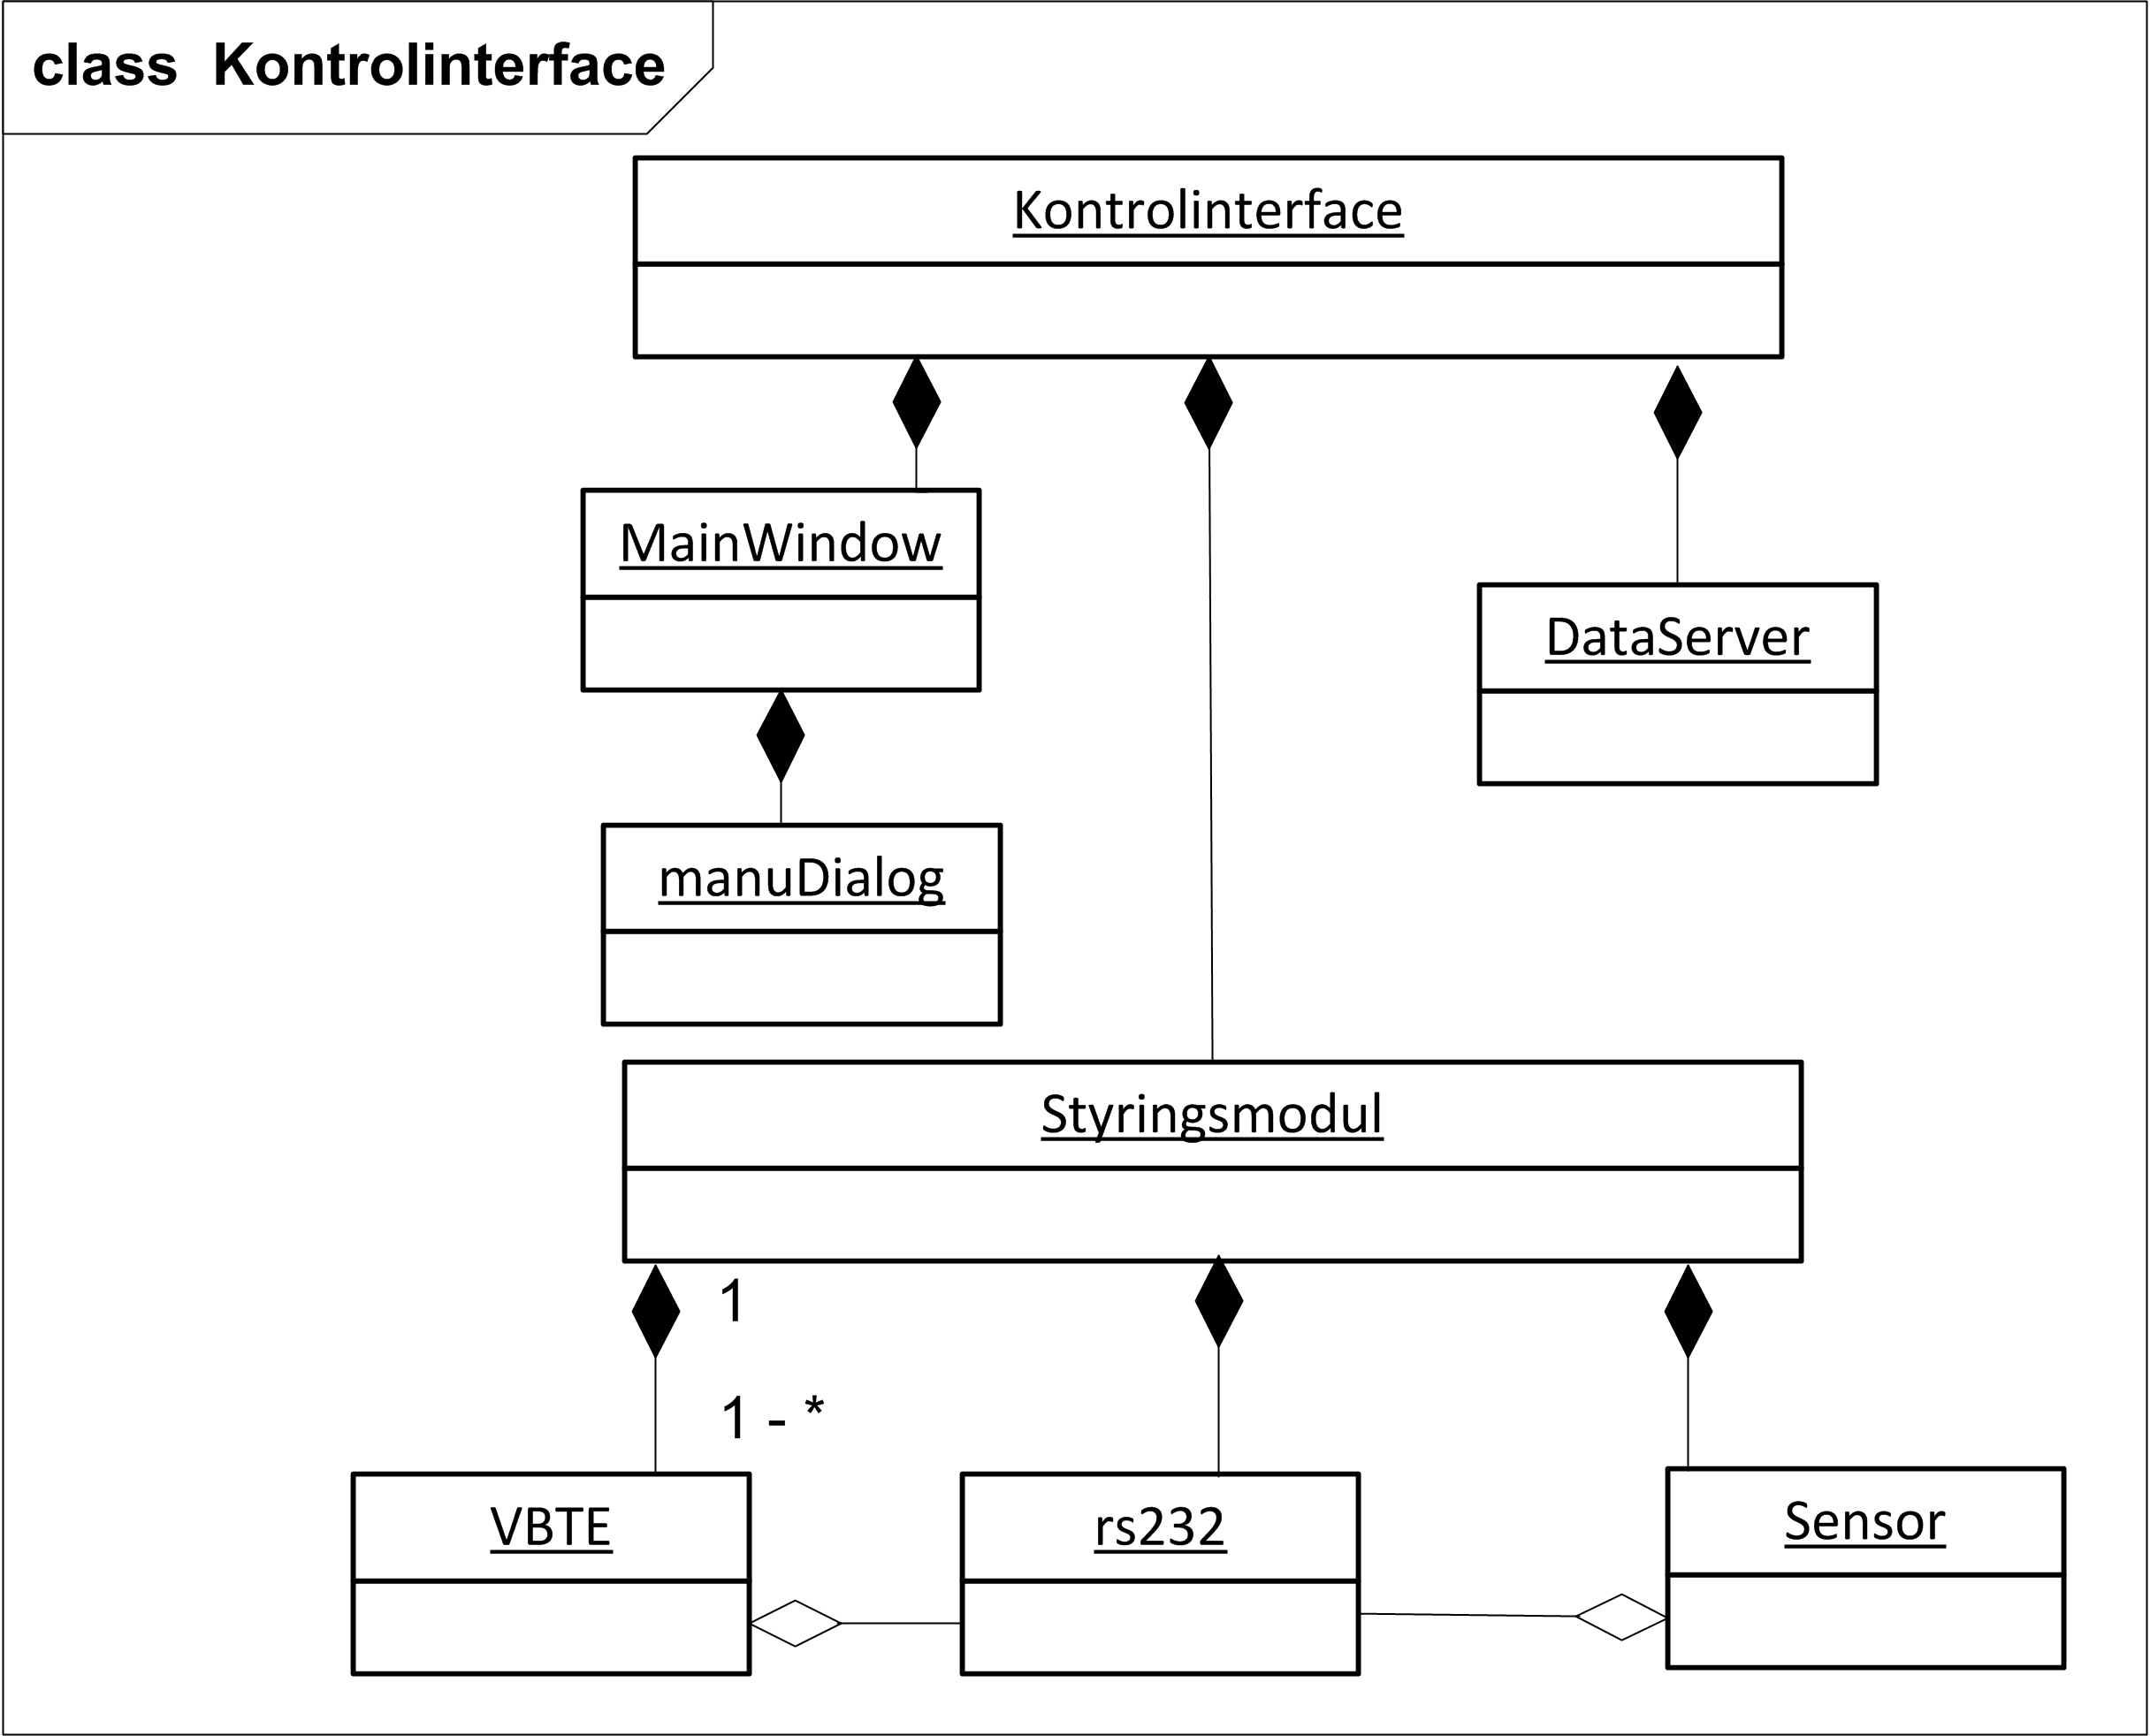
\includegraphics[width=1\textwidth]{billeder/GUI/klassediagram_simpel}
\caption{På figuren ses det simple klassediagram for Kontrolinterfacet. Se en beskrivelse af hver klasse i tabel \ref{tabel:ki-klasser}}
\end{figure}

En beskrivelse af hver klasse kan findes i tabel \ref{tabel:ki-klasser}.\\
 
\begin{table}[H]
\centering
\rowcolors{1}{white}{light-gray}
\begin{tabular}{| p{3cm}  p{12.5cm}|}
\multicolumn{2}{l}{{\Large Kontrolinterfacets klasser}} \\\hline
Kontrolinterface:&Programmets hovedklasse. Eksisterer for at rydde op i main-funktionen.\\\hline
DataServer:&Står for alt TCP-kommunikationen med databasen. Oprettes af KI-klassen\\\hline
Styringsmodul:&Oprettes af KI og opretter VBTE-, Sensor- og RS232klasserne.\\\hline
Sensor:&Oprettes af SM og er ansvarlig for hældningsværdien.\\\hline
VBTE:&Der eksisterer et VBTE-objekt for hvert fysisk VBTE-modul. Det er objektets ansvar at holde styr på værdierne for sit VBTE-modul.\\\hline
RS232:&Objektet oprettes af SM-klassen og VBTE- og Sensorobjekterne har en delt association til den. Objektet har ansvaret for kommunikationen med det fysiske SM-modul. Objektet formidler sig på en protokol forstået den kommunikationsansvarlige kode på SM-modulet. Protokollen kan ses i dokumentet for det detaljerede softwaredesign.\\\hline
MainWindow:&Oprettes af KI-klassen. Kontrollerer og overvåger den grafiske brugergrænsefalde.\\\hline
manudialog:&Oprettes af MainWindow og styrer den dialog, der fremkommer når man ønsker en manuel hældningsregulering.\\\hline
\end{tabular}
\caption{Kontrolinterfacets klasser}
\label{tabel:ki-klasser}
\end{table}

Der er så udarbejdet et detaljeret klassediagram for klasserne i Kontrolinterfacet. Dette udarbejdes ud fra det detaljerede state machine diagram og de krav der er stillet i kravspecifikationen. Brugergrænsefladen udarbejdes ud fra de modeller der er aftalt med kunden og som ligger som bilag A i kravspecifikationen.\\
Det detaljerede klassediagram indeholder de samme klasser og relationer som det simplificerede. Derudover er der anført hvilke metoder, signaler, slots og attributter klasserne indeholder. \\
Signaler og slots er indført af Qt-frameworket og muliggør kommunikation mellem klasser uden at koble klasserne unødvendig meget. En klasse abbonnerer så at sige på et signal. Udsendes signalet så vil funktionaliteten i en slot så blive kaldt. Flere klasser kan godt reagerer på samme signal. Således kan et signal godt påvirke flere elementer af programmet.\\
Derudover er de anvendte enumeratorer og structs indført i diagrammet. Structs er indført i designet for at kunne pakke flere værdier ned og sende dem samtidigt. Enumerationer gør koden nemmere at læse og gør det nemt at implementere en protokol som fx protokol til Styringsmodulet.\\
Bemærk at klassediagrammet er delt op i to. Skæringsstedet er mellem Kontrolinterface-klassen og Styringsmodul-klassen og er markeret med <<extend>>.\\
Klassediagrammet for Kontrolinterface-klassen og de tilhørende klasser kan ses på figur \ref{fig:kd_ki_del} og for Styringsmodul-delen henvises der til figur \ref{fig:kd_sm_del}.

\begin{figure}[H]
\centering
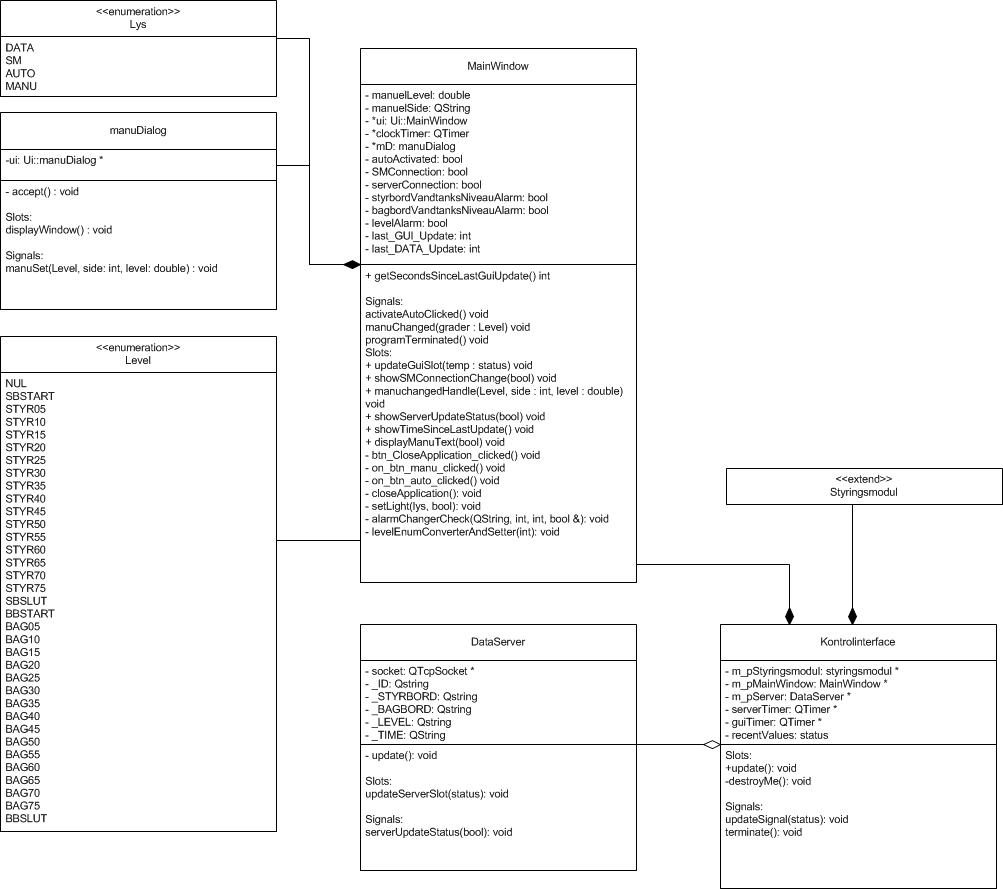
\includegraphics[width=1\textwidth]{billeder/KI-Class}
\caption{På figuren ses klassediagrammet for KI - Kontrolinterface-delen}
\label{fig:kd_ki_del}
\end{figure}

\begin{figure}[H]
\centering
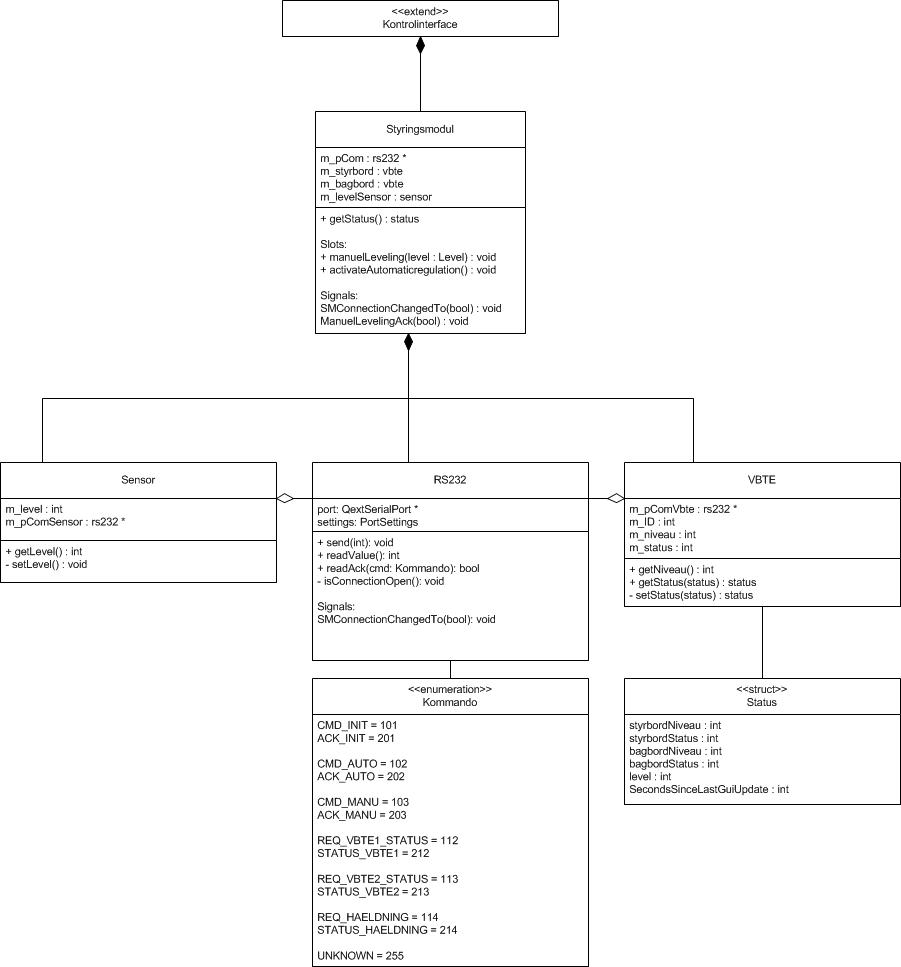
\includegraphics[width=1\textwidth]{billeder/SM-Class}
\caption{På figuren ses klassediagrammet for KI - Styringsmodul-delen}
\label{fig:kd_sm_del}
\end{figure}

\section{Metode- og klassebeskrivelser}
Når klassediagrammet er på plads skal metoderne i det beskrives. Det vil de blive gjort i dette afsnit.

\subsection{MainWindow}
\subsubsection{Ansvar}
Denne klasse indeholder de funktioner der er skrevet til Qt-formen MainWindow.ui hvori selve det grafiske er opbygget. Klassen indeholder de funktioner der anvendes i forbindelse med den grafiske brugergrænseflade. Det være sig når der kommer et input, eller der skal opdateres nogle værdier på skærmen.
\subsubsection{Funktionsbeskrivelser}
 
\begin{table}[H]
\begin{tabular}{l p{12.5cm}}
\multicolumn{2}{l}{\texttt{\textcolor{blue}{int} getSecondsSinceLastGuiUpdate();}} \\
\hline
Beskrivelse:& En simpelt get-funktionen der returnerer værdien af klasseattributten \textit{last\_GUI\_Update.} \\
Parametre:&Ingen\\
Returværdi:&\texttt{\textcolor{blue}{int} secondsSinceLastGuiUpdate}\\
\end{tabular}
\end{table}

\begin{table}[H]
\begin{tabular}{l p{12.5cm}}
\multicolumn{2}{l}{\texttt{\textcolor{blue}{void} updateGuiSlot(\textcolor{blue}{status} temp);}} \\
\hline
Beskrivelse:& Bliver kaldt når GUI'en skal opdateres. 
Den modtager parameterent \textit{temp} som er en struct af typen status. 
Ud fra denne struct hives de værdier ud, som skal vises på GUI'en. Værdierne vises ved de set-funktioner der er tilknyttet de anvendte widgets (og dermed en del af Qt-frameworket.) 
Når værdierne er opdateret vises det som en aktivitet i aktivitetsloggen \\   
Parametre:&\texttt{\textcolor{blue}{status} temp}\\
Returværdi:&Ingen\\
\end{tabular}
\end{table}

\begin{table}[H]
\begin{tabular}{l p{12.5cm}}
\multicolumn{2}{l}{\texttt{\textcolor{blue}{void} showSMConnectionChange();}} \\
\hline
Beskrivelse:& Kaldes hvis SM-forbindelsen til styringsmodulet ændres fra forbundet til mistet forbindelse eller omvendt. Det udløser en aktivitet i aktivitetsloggen. Derudover skiftes lyset på gui'en. Parameteren state er den status som forbindelsen har ændret sig til.\\   
Parametre:&\texttt{\textcolor{blue}{bool} state}\\
Returværdi:&Ingen\\
\end{tabular}
\end{table}

\begin{table}[H]
\begin{tabular}{l p{12.5cm}}
\multicolumn{2}{l}{\texttt{\textcolor{blue}{void} manuChangedHandle(\textcolor{blue}{Level} samlet, \textcolor{blue}{int} side, \textcolor{blue}{double} level);}} \\
\hline
Beskrivelse:& Kaldes når brugeren har ændret i indstillingen til den manuelle hældning. Som parametre modtages hvilken side man ønsker at skibet skal hælde til (int side), hvor meget det skal hælde (double level) samt de to informationer samlet i en enum, Level samlet.
Funktionen emitter signalet "manuChanged(Level temp). Det sætter også klasseattributerne manuelSide, manuelLevel samt autoActivated til deres rette værdier.
Til sidst kaldes funktionen displayManuText(true)\\   
Parametre:&\texttt{\textcolor{blue}{Level} samlet}\\
&\texttt{\textcolor{blue}{int} side}\\
&\texttt{\textcolor{blue}{double} level}\\
Returværdi:&Ingen\\
\end{tabular}
\end{table}


\begin{table}[H]
\begin{tabular}{l p{12.5cm}}
\multicolumn{2}{l}{\texttt{\textcolor{blue}{void} showServerUpdateStatus(\textcolor{blue}{bool} state);}} \\
\hline
Beskrivelse:&Kaldes hver gang signalet DataServer::serverUpdateStatus() udsendes. Funktionen undersøger om forbindelsen har ændret sig ved at sammenligne med attributen serverConnection.
Hvis forbindelsen har ændret sig udsendes dette som en aktivitet. Lyset ændres også således at det passer ved hjælp af setLight(DATA, serverConnection. Hvis vi modtager "true" vil last\_DATA\_Update opdateres til således til den nuværende værdi af sekunder siden epoch.\\   
Parametre:&Ingen\\
Returværdi:&Ingen\\
\end{tabular}
\end{table}


\begin{table}[H]
\begin{tabular}{l p{12.5cm}}
\multicolumn{2}{l}{\texttt{\textcolor{blue}{void} showTimeSinceLastUpdate();}} \\
\hline
Beskrivelse:&Kaldes hvert sekund. Funktionen opdaterer antallet af sekunder siden sidste overførelse af data til serveren eller til SM. Når tiden er længere end tiden mellem hver opdatering vil dette tal skifte til rødt.\\    
Parametre:&Ingen\\
Returværdi:&Ingen\\
\end{tabular}
\end{table}


\begin{table}[H]
\begin{tabular}{l p{12.5cm}}
\multicolumn{2}{l}{\texttt{\textcolor{blue}{void} displayManuText(\textcolor{blue}{bool} show);}} \\
\hline
Beskrivelse:&Viser eller skjuler teksten med indstillingen af manuel hældning afhængig af parameteret show.\\    
Parametre:&Ingen\\
Returværdi:&Ingen\\
\end{tabular}
\end{table}



\begin{table}[H]
\begin{tabular}{l p{12.5cm}}
\multicolumn{2}{l}{\texttt{\textcolor{blue}{void} activateAutoClicked();}} \\
\hline
Beskrivelse:& udsendes når der er blevet trykket på knappen \textit{activateAutoClicked}\\
Parametre:&Ingen\\
Returværdi:&Ingen\\
\end{tabular}
\end{table}


\begin{table}[H]
\begin{tabular}{l p{12.5cm}}
\multicolumn{2}{l}{\texttt{\textcolor{blue}{void} activateAutoClicked();}} \\
\hline
Beskrivelse:& udsendes når der er blevet trykket på knappen \textit{activateAutoClicked}\\
Parametre:&Ingen\\
Returværdi:&Ingen\\
\end{tabular}
\end{table}


\begin{table}[H]
\begin{tabular}{l p{12.5cm}}
\multicolumn{2}{l}{\texttt{\textcolor{blue}{void} manuChanged(\textcolor{blue}{Level} grader);}} \\
\hline
Beskrivelse:&Udsendes når der er blevet ændret en manuel indstilling.\\
Parametre:&\texttt{\textcolor{blue}{Level} grader}\\
Returværdi:&Ingen\\
\end{tabular}
\end{table}


\begin{table}[H]
\begin{tabular}{l p{12.5cm}}
\multicolumn{2}{l}{\texttt{\textcolor{blue}{void} programTerminated();}} \\
\hline
Beskrivelse:&Udsendes når programmet er blevet lukket ned.\\
Parametre:&Ingen\\
Returværdi:&Ingen\\
\end{tabular}
\end{table}

\begin{table}[H]
\begin{tabular}{l p{12.5cm}}
\multicolumn{2}{l}{\texttt{\textcolor{blue}{void} btn\_CloseApplication\_clicked();}} \\
\hline
Beskrivelse: &Kaldes når luk-knappen på GUI'en er blevet trykket. 
Udsender signalet programTerminated() hvis brugeren bekræfter valget\\
Parametre:&Ingen\\
Returværdi:&Ingen\\
\end{tabular}
\end{table}

\begin{table}[H]
\begin{tabular}{l p{12.5cm}}
\multicolumn{2}{l}{\texttt{\textcolor{blue}{void} on\_btn\_manu\_clicked();}} \\
\hline
Beskrivelse: &Kaldes når der bliver trykket på knappen for manuel hældning. Viser dialogen "manuDialog".\\
Parametre:&Ingen\\
Returværdi:&Ingen\\
\end{tabular}
\end{table}

\begin{table}[H]
\begin{tabular}{l p{12.5cm}}
\multicolumn{2}{l}{\texttt{\textcolor{blue}{void} on\_btn\_auto\_clicked();
}} \\
\hline
Beskrivelse:&Kaldes når der trykkes på \textit{Automatisk Hældnings-knappen}. Aktiverer automatisk styring og deaktiverer den manuelle.\\
Parametre:&Ingen\\
Returværdi:&Ingen\\
\end{tabular}
\end{table}

\begin{table}[H]
\begin{tabular}{l p{12.5cm}}
\multicolumn{2}{l}{\texttt{\textcolor{blue}{void} setLight(\textcolor{blue}{lys} id, \textcolor{blue}{bool} state);}} \\
\hline
Beskrivelse:&Sætter lyset i forhold til parametrene. lys er en enum der bestemmer hvilket element lyset skal ændres for. state er om lyset skal være tændt eller ej\\
Parametre:&\texttt{\textcolor{blue}{lys} id}\\
&\texttt{\textcolor{blue}{bool} state}\\
Returværdi:&Ingen\\
\end{tabular}
\end{table}

%\multicolumn{2}{l}{\texttt{\textcolor{blue}{void} alarmChangerCheck(QString sentence, int critical\_point, int value, bool &earlier\_state);}} \\

\begin{table}[H]
\begin{tabular}{l p{12.5cm}}
\multicolumn{2}{l}{\texttt{\textcolor{blue}{void} alarmChangerCheck(\textcolor{blue}{QString} sentence, \textcolor{blue}{int} critical\_point, \textcolor{blue}{int} value, \textcolor{blue}{bool} \&earlier\_state);}} \\
\hline
Beskrivelse: &Tester om alarmerne har ændret sig. Sentence er starten af den sætning der skrives i aktivitetsloggen. critical\_point er det kritiske punkt for det emne der arbejdes på. Value er den værdi den har. Earlier\_state er hvilket stadie alarmen var i tidligere.\\
Parametre:&\texttt{\textcolor{blue}{QString} sentence}\\
&\texttt{\textcolor{blue}{int} critical\_point}\\
&\texttt{\textcolor{blue}{int} value}\\
&\texttt{\textcolor{blue}{bool} \&earlier\_state}\\
Returværdi:&Ingen\\
\end{tabular}
\end{table}

\begin{table}[H]
\begin{tabular}{l p{12.5cm}}
\multicolumn{2}{l}{\texttt{\textcolor{blue}{void} levelEnumConverterAndSetter(\textcolor{blue}{int} level);}} \\
\hline
Beskrivelse: &Konverterer en integer baseret på Level-enumeratoren om til en side og en vinkel.\\
Parametre:&\texttt{\textcolor{blue}{int} level}\\
Returværdi:&Ingen\\
\end{tabular}
\end{table}


\subsection{Kontrolinterface}
\subsubsection{Ansvar}
Dette er hovedklassen hvori selve programmet lever. Oprettelsen af et objekt af denne klasse er derfor også det eneste der sker i main.
\subsubsection{Funktionsbeskrivelser}

\begin{table}[H]
\begin{tabular}{l p{12.5cm}}
\multicolumn{2}{l}{\texttt{\textcolor{blue}{void} update();}} \\
\hline
Beskrivelse: &Får en status-struct fra SM-klassen udfyldt med de nuværende værdier for systemet. Tilføjer antal sekunder siden sidste gui-update ved hjælp af getSecondsSinceLastGuiUpdate. Denne struct udsendes med signalet updateSignal(status recentValues)\\
Parametre:&Ingen\\
Returværdi:&Ingen\\
\end{tabular}
\end{table}

\begin{table}[H]
\begin{tabular}{l p{12.5cm}}
\multicolumn{2}{l}{\texttt{\textcolor{blue}{void} updateSignal(\textcolor{blue}{status} recentValues);}} \\
\hline
Beskrivelse: &Signalet der sendes når gui og server skal updateres. Indeholder en struct med alle relevante værdier.\\
Parametre:&\texttt{\textcolor{blue}{status} recentValues}\\
Returværdi:&Ingen\\
\end{tabular}
\end{table}

\begin{table}[H]
\begin{tabular}{l p{12.5cm}}
\multicolumn{2}{l}{\texttt{\textcolor{blue}{void} terminate();}} \\
\hline
Beskrivelse: &Udsendes når brugeren ønsker at terminere programmet.\\
Parametre:&Ingen\\
Returværdi:&Ingen\\
\end{tabular}
\end{table}

\begin{table}[H]
\begin{tabular}{l p{12.5cm}}
\multicolumn{2}{l}{\texttt{\textcolor{blue}{void} destroyMe();}} \\
\hline
Beskrivelse: &Muliggør nedlæggelse af klassen med et funktionskald.\\
Parametre:&Ingen\\
Returværdi:&Ingen\\
\end{tabular}
\end{table}

\subsection{DataServer}
\subsubsection{Ansvar}
Klassen står for al kommunikation med serveren via en TCP-forbindelse. Forbindelse oprettes og nedlægges hver gang der tages kontakt. DataServer-objektet opdaterer serveren når den får ordre om det fra Kontrolinterface-klassen.
\subsubsection{Funktionsbeskrivelser}

\begin{table}[H]
\begin{tabular}{l p{12.5cm}}
\multicolumn{2}{l}{\texttt{\textcolor{blue}{void} onDelete();}} \\
\hline
Beskrivelse: &Kaldes i destruktoren. Sender en besked til serveren om at programmet termineres	.\\
Parametre:&Ingen\\
Returværdi:&Ingen\\
\end{tabular}
\end{table}

\begin{table}[H]
\begin{tabular}{l p{12.5cm}}
\multicolumn{2}{l}{\texttt{\textcolor{blue}{void} updateServerSlot(\textcolor{blue}{status} recentValues);}} \\
\hline
Beskrivelse: &Kaldes når signalet updateSignal(status recentValues) udsendes. Funktionen sørger så for at der via TCP-forbindelsen bliver udsendt de relevante værdier til databasen.\\
Parametre:&\texttt{\textcolor{blue}{status} recentValues}\\
Returværdi:&Ingen\\
\end{tabular}
\end{table}

\begin{table}[H]
\begin{tabular}{l p{12.5cm}}
\multicolumn{2}{l}{\texttt{\textcolor{blue}{void} serverUpdateStatus(\textcolor{blue}{bool} status);}} \\
\hline
Beskrivelse: &Udsendes når databasen er blevet opdateret. Parameteren "status" indikerer hvorvidt overførelsen var succesfuld eller ej. Der ventes ikke noget svar fra databasen.\\
Parametre:&\texttt{\textcolor{blue}{bool} status}\\
Returværdi:&Ingen\\
\end{tabular}
\end{table}



\subsection{manuDialog}
\subsubsection{Ansvar}
manuDialog-klassen står for håndtering af det vindue der åbnes ved tryk på \textit{Manuel Hældningsregulering-knappen}.
\subsubsection{Funktionsbeskrivelser}

\begin{table}[H]
\begin{tabular}{l p{12.5cm}}
\multicolumn{2}{l}{\texttt{\textcolor{blue}{void} manuSet(\textcolor{blue}{Level} degrees, \textcolor{blue}{int} side, \textcolor{blue}{double} level);}} \\
\hline
Beskrivelse: &Udsendes i funktionen accept(). Der medsendes de data som brugeren har valgt på dialogen.\\
Parametre:&\texttt{\textcolor{blue}{Level} degrees}\\
&\texttt{\textcolor{blue}{int} side}\\
&\texttt{\textcolor{blue}{double} level}\\
Returværdi:&Ingen\\
\end{tabular}
\end{table}

\begin{table}[H]
\begin{tabular}{l p{12.5cm}}
\multicolumn{2}{l}{\texttt{\textcolor{blue}{void} accept();}} \\
\hline
Beskrivelse: &Kaldes når der trykkes på "OK"-knappen på dialogen. Det indtastede omdannes til en værdi i forhold til enumeratoren "Level". Dialogen lukkes og signalet manuSet(...) udsendes \\
Parametre:&\texttt{\textcolor{blue}{Level} degrees}\\
&\texttt{\textcolor{blue}{int} side}\\
&\texttt{\textcolor{blue}{double} level}\\
Returværdi:&Ingen\\
\end{tabular}
\end{table}

\subsection{Styringsmodul}
\subsubsection{Ansvar}
Klassen har samme rolle som det fysiske styringsmodul har i systemet. Det giver kontrolinterfacet adgang til sensor-værdier og vandstandsniveauer igennem sine underklasser, VBTE og Sensor.
\subsubsection{Funktionsbeskrivelser}

\begin{table}[H]
\begin{tabular}{l p{12.5cm}}
\multicolumn{2}{l}{\texttt{\textcolor{blue}{status} getStatus();}} \\
\hline
Beskrivelse: &Indhenter værdierne for systemet fra VBTE'er og Hældningssensor. Disse værdier sættes ind i structen temp som så returneres.\\
Parametre:&Ingen\\
Returværdi:&\texttt{\textcolor{blue}{status} recentValues}\\
\end{tabular}
\end{table}

\begin{table}[H]
\begin{tabular}{l p{12.5cm}}
\multicolumn{2}{l}{\texttt{\textcolor{blue}{void} manuelLeveling(\textcolor{blue}{Level} level);}} \\
\hline
Beskrivelse: &Sender kommando og vinkel til PSoC over RS232 vha. objektet m\_pCom.\\
Parametre:&\texttt{\textcolor{blue}{Level} level}\\
Returværdi:&Ingen\\
\end{tabular}
\end{table}


\begin{table}[H]
\begin{tabular}{l p{12.5cm}}
\multicolumn{2}{l}{\texttt{\textcolor{blue}{void} activateAutomaticRegulation();}} \\
\hline
Beskrivelse: &Sætter hvorvidt automatisk regulering skal være aktiveret eller ej til styringsmodulet.\\
Parametre:&Ingen\\
Returværdi:&Ingen\\
\end{tabular}
\end{table}

\begin{table}[H]
\begin{tabular}{l p{12.5cm}}
\multicolumn{2}{l}{\texttt{\textcolor{blue}{void} SMConnectionChangedTo(\textcolor{blue}{bool} status);}} \\
\hline
Beskrivelse: &Udsendes hver gang der har været en overførelse. Status indikerer hvorvidt overførelsen var succesfuld eller ej.\\
Parametre:&\texttt{\textcolor{blue}{bool} status}\\
Returværdi:&Ingen\\
\end{tabular}
\end{table}

\begin{table}[H]
\begin{tabular}{l p{12.5cm}}
\multicolumn{2}{l}{\texttt{\textcolor{blue}{void} ManuelLevelingAck(\textcolor{blue}{bool} status);}} \\
\hline
Beskrivelse: &Udsendes når der er blevet sendt kommandoen CMD\_MANU til styringsmodulet. Bool status indikerer hvorvidt overførelsen var succesfuld ej.\\
Parametre:&\texttt{\textcolor{blue}{bool} status}\\
Returværdi:&Ingen\\
\end{tabular}
\end{table}

\subsection{VBTE}
\subsubsection{Ansvar}
Håndterer værdierne for hver sin vandballasttankenhed. Kommunikerer til det fysiske styringsmodul ved hjælp af RS232-klassen.
\subsubsection{Funktionsbeskrivelser}

\begin{table}[H]
\begin{tabular}{l p{12.5cm}}
\multicolumn{2}{l}{\texttt{\textcolor{blue}{int} getNiveau();}} \\
\hline
Beskrivelse: &Kalder setNiveau og returnerer værdien af niveau\\
Parametre:&Ingen\\
Returværdi:&\textcolor{blue}{int} niveau()\\
\end{tabular}
\end{table}

\begin{table}[H]
\begin{tabular}{l p{12.5cm}}
\multicolumn{2}{l}{\texttt{\textcolor{blue}{status} getStatus(\textcolor{blue}{status} temp);}} \\
\hline
Beskrivelse: &Skaffer status vha. rs232-objektet og sætter niveau og status i structen temp som herefter returneres.\\
Parametre:&\textcolor{blue}{status} temp()\\
Returværdi:&\textcolor{blue}{status} temp()\\
\end{tabular}
\end{table}

\subsection{Sensor}
\subsubsection{Ansvar}
Håndterer værdierne for hældningssensoreren. Kommunikerer til det fysiske styringsmodul ved hjælp af RS232-klassen.
\subsubsection{Funktionsbeskrivelser}

\begin{table}[H]
\begin{tabular}{l p{12.5cm}}
\multicolumn{2}{l}{\texttt{\textcolor{blue}{int} getLevel();}} \\
\hline
Beskrivelse: &Skaffer værdien af hældningen på skibet vha. rs232-objektet og returnerer det.\\
Parametre:&Ingen\\
Returværdi:&\textcolor{blue}{int} level\\
\end{tabular}
\end{table}

\subsection{RS232}
\subsubsection{Ansvar}
Håndterer kommunikationen til det fysiske styringsmodul ved protokollen der ses i enumeratoren "Kommando". 
\subsubsection{Funktionsbeskrivelser}

\begin{table}[H]
\begin{tabular}{l p{12.5cm}}
\multicolumn{2}{l}{\texttt{\textcolor{blue}{void} send(\textcolor{blue}{int} cmd);}} \\
\hline
Beskrivelse: &Sendefunktion. Sender den medsendte integer.\\
Parametre:&\textcolor{blue}{int} cmd\\
Returværdi:&Ingen\\
\end{tabular}
\end{table}

\begin{table}[H]
\begin{tabular}{l p{12.5cm}}
\multicolumn{2}{l}{\texttt{\textcolor{blue}{int} readValue();}} \\
\hline
Beskrivelse: &Modtagerfunktion. Returnerer den læste værdi.\\
Parametre:&Ingen\\
Returværdi:&\textcolor{blue}{int} receivedValue\\
\end{tabular}
\end{table}

\begin{table}[H]
\begin{tabular}{l p{12.5cm}}
\multicolumn{2}{l}{\texttt{\textcolor{blue}{bool} readAck(\textcolor{blue}{Kommando} cmd);}} \\
\hline
Beskrivelse: &Kalder readValue() og sammenholder dennes returværdi med den værdi der er medsendt som parameter (cmd). Returnerer hvor vidt de to var identiske.\\
Parametre:&\textcolor{blue}{Kommando} cmd\\
Returværdi:&\textcolor{blue}{bool} status\\
\end{tabular}
\end{table}

\begin{table}[H]
\begin{tabular}{l p{12.5cm}}
\multicolumn{2}{l}{\texttt{\textcolor{blue}{void} SMConnectionChangedTo(\textcolor{blue}{bool} status);}} \\
\hline
Beskrivelse: &Når der har været en overførelse udsendes dette signal. Status indikerer hvorvidt overførelsen var succesfuld eller ej.\\
Parametre:&\textcolor{blue}{bool} status\\
Returværdi:&Ingen\\
\end{tabular}
\end{table}

\begin{table}[H]
\begin{tabular}{l p{12.5cm}}
\multicolumn{2}{l}{\texttt{\textcolor{blue}{void} SMConnectionChangedTo(\textcolor{blue}{bool} status);}} \\
\hline
Beskrivelse: &Når der har været en overførelse udsendes dette signal. Status indikerer hvorvidt overførelsen var succesfuld eller ej.\\
Parametre:&\textcolor{blue}{bool} status\\
Returværdi:&Ingen\\
\end{tabular}
\end{table}

\begin{table}[H]
\begin{tabular}{l p{12.5cm}}
\multicolumn{2}{l}{\texttt{\textcolor{blue}{bool} isConnectionOpen();}} \\
\hline
Beskrivelse: &Tester om der er forbindelse til PSoC\\
Parametre:&Ingen\\
Returværdi:&\textcolor{blue}{bool} connectionState\\
\end{tabular}
\end{table}